\chapter{SQL}

\section{Interrogazione di una base dati}
L'interrogazione di una base di dati è uno degli aspetti più importanti del linguaggio SQL.\
I comandi di interrogazione, o \textbf{QUERY}, permettono di effettuare una ricerca dei dati presenti nel database che soddisfano particolari condizioni richieste dall'utente.

SQL è stato definito nel 1973 ed è oggi il linguaggio universale dei sistemi relazionali.\
SQL è un calcolo su \textbf{multi-insiemi} e il suo comando base è
\begin{flushleft}
	\texttt{SELECT [DISTINCT] Attributo \{Attributo\}}

	\quad \texttt{FROM Tabella [Ide] \{Tabella [Ide]\}}

	\quad \texttt{[WHERE Condizione]}
\end{flushleft}

\noindent Semantica:\ prodotto + restrizione + proiezione.\
Un attributo A di una tabella ``$R\ x$'' si denota come $A$ oppure $R.A$ oppure $x.A$.

\subsubsection{Istruzione SELECT per l'interrogazione}

Le query vengono effettuate mediante il comando \texttt{SELECT}.\
Sintassi:
\begin{flushleft}
	\texttt{SELECT ListaAttributi}

	\texttt{FROM ListaTabelle}

	\texttt{[ WHERE Condizione ]}
\end{flushleft}

\noindent Bisogna specificare:
\begin{itemize}
	\item la ``target list'' cioè la lista degli attributi interessati;
	\item clausola \texttt{FROM} per stabilire in quale/quali tabella/e sono contenuti i dati che ci occorrono;
	\item clausola \texttt{WHERE} per esprimere le condizioni che i dati cercati devono soddisfare.
\end{itemize}

\subsubsection{Target List (lista degli attributi)}

Specificare la target list corrisponde a scegliere alcuni degli attributi della tabella o delle tabelle considerate.\
Implementa l'operazione di \textbf{proiezione} dell'algebra relazionale.

Se si desidera visualizzare tutti gli attributi della tabella, si può semplificare la target list indicando la lista con un semplice asterisco *.\
\subsubsection{Where}

La clausola \texttt{WHERE} serve a scegliere le righe della tabella che soddisfano una certa condizione.\
In questo modo la clausola \texttt{where} implementa la \textbf{selezione} dell'algebra relazionale.\
Ovviamente la clausola \texttt{WHERE} è opzionale, e se si omette, si selezionano tutte le righe della tabella specificata.

\subsubsection{From}

La clausola \texttt{FROM} ha lo scopo di scegliere quali sono le tabelle del database da cui vogliamo estrarre le nostre informazioni.\
Nel caso in cui le tabelle elencate sono due, la clausola \texttt{FROM}, insieme con la clausola \texttt{WHERE}, che stabilisce quali righe delle due tabelle bisogna accoppiare, implementa il \textbf{theta join}.

\subsubsection{Select}
\begin{table}[H]
	\centering
	\begin{tabular}{l}
		\texttt{SELECT ListaAttributi} \\
		\texttt{FROM ListaTabelle}     \\
		\texttt{[WHERE Condizione]}    \\
	\end{tabular}
\end{table}
La query considera il prodotto cartesiano tra le tabelle in \texttt{ListaTabelle} (\textit{join}).\
Fra queste seleziona solo le righe che soddisfano la \texttt{Condizione} (\textit{selezione}) e infine valuta le espressioni specificate nella target list \texttt{ListaAttri\-buti} (\textit{proiezione}).\
La \texttt{SELECT} implementa quindi gli operatori di proiezione, selezione e join dell'algebra relazionale.\

\newpage

\subsubsection{La lista degli attributi}
Attributi ::= * $|$ Expr [\texttt{[AS] nuovoNome}] \{Expr [\texttt{[AS] nuovoNome}]\}

\noindent Expr ::= [Ide.]Attributo $|$ Const $|$ (Expr) $|$ [-] Expr [Op Expr] $|$ \texttt{COUNT}(*) $|$ AggrFun ([\texttt{DISTINCT}] [Ide.]Attributo)

\noindent e \texttt{AS x}:\ dà un nome a una colonna.

\noindent e AggrFun ::= $ \mathtt{SUM}\ |\ \mathtt{COUNT}\ |\ \mathtt{AVG}\ |\ \mathtt{MAX}\ |\ \mathtt{MIN}$

\noindent AggrFun:\ o si usano tutte funzioni di aggregazione (e si ottiene un'unica riga) o non se ne usa nessuna.

\subsubsection{La lista delle tabelle}
Le tabelle si possono combinare usando `\texttt{,}' (prodotto):\ $\mathtt{FROM\ T_1,T_2}$.

Giunzioni di vario genere:
\begin{itemize}
	\item Studenti s \texttt{JOIN} Esami e \texttt{ON} s.Matricola=e.Matricola
	\item Studenti s \texttt{JOIN} Esami e \texttt{USING} Matricola
	\item Studenti s \texttt{NATURAL JOIN} Esami e
	\item Studenti s \texttt{LEFT JOIN} Esami e \texttt{ON} s.Matricola=e.Matricola
	\item \texttt{LEFT JOIN - USING}
	\item \texttt{NATURAL LEFT JOIN}
	\item \texttt{RIGHT JOIN}
	\item \texttt{FULL JOIN}
\end{itemize}

\subsubsection{La condizione}

Combinazione booleana di predicati tra cui:
\begin{itemize}
	\item Expr Comp Expr
	\item Expr Comp (Sottoselect che torna un valore)
	\item \texttt{[NOT] EXISTS} (Sottoselect)
	\item Espr Comp (\texttt{ANY} $|$ \texttt{ALL}) (Sottoselect)
	\item Expr \texttt{[NOT] IN} (Sottoselect) (oppure $\mathtt{IN (v\textsubscript{1},\ \dots,v\textsubscript{n})}$)
\end{itemize}
Comp:\ $<,\ =,\ >,\ \neq,\ \leq,\ \geq$

\noindent Connettori logici \texttt{AND}, \texttt{OR}, \texttt{NOT}.\
\newpage
\noindent Operatori:\ \texttt{BETWEEN} consente la selezione di righe con attributi in un particolare
range, \texttt{IN} è usato per selezionare righe che hanno un attributo che assume valori contenuti in una lista, \texttt{LIKE} è usato per effettuare ricerche ``wildcard'' (ossia con un simbolo jolly) di una stringa di valori.\ Le condizioni di ricerca possono contenere letterali, caratteri o numeri.\
Esistono due tipi di wildcard:
\begin{itemize}
	\item `\%' denota zero o più caratteri.
	\item `\_' denota un carattere
\end{itemize}
A volte può succedere che uno dei simboli coinvolti nel pattern matching sia proprio `\_' oppure `\%'.\
In questo caso, si sceglie un simbolo che non è ammesso fra i simboli della stringa (supponiamo `\#') detto simbolo escape, nell'espressione per la ricerca si fa precedere il simbolo `\_' o `\%' cercato dal simbolo escape, e poi si specifica che `\#' è il simbolo di escape.

Il valore di un campo di un'ennupla può mancare per varie ragioni; SQL fornisce il valore speciale \texttt{NULL} per tali situazioni.\
La presenza del \texttt{NULL} introduce dei problemi:
\begin{itemize}
	\item occorrono dei predicati per controllare se un valore è/non è \texttt{NULL}.
	\item la condizione ``reddito $>$ 8'' è vera o falsa quando il reddito è uguale a \texttt{NULL}?\ Cosa succede degli operatori \texttt{AND}, \texttt{OR} e \texttt{NOT}?
	\item Occorre una logica a 3 valori (vero, falso e unknown).
	\item Va definita opportunamente la semantica dei costrutti.\ Ad esempio il \texttt{WHERE} elimina le ennuple che non rendono vera la condizione.
\end{itemize}
L'operatore \texttt{IS NULL} verifica se il contenuto di un operando è \texttt{NULL}.\

Tutti gli operatori descritti sono presenti anche in forma negativa, con ovvio significato.

\subsubsection{Alias delle colonne}
L'alias serve a dare a una colonna un nome diverso rispetto a quello che è utilizzato nella definizione della tabella.\
Implementa l'operatore $\rho$ (\textit{ridenominazione}) dell'algebra relazionale.

Può essere usata opzionalmente la parola chiave \texttt{AS} tra il nome della colonna e l'alias richiede necessariamente le virgolette se l'alias ha degli spazi.

\section{Ordinamento, Operatori aggregati e Raggruppamento}

\subsection{Ordinamento del risultato}

È possibile dare un ordinamento del risultato di una \texttt{Select}.\
L'ordinamento si può effettuare in base a un attributo e può essere crescente o decrescente.\
La sintassi è la seguente:

\begin{flushleft}
	\texttt{SELECT lista\_attributi}

	\texttt{FROM nome\_tabella}

	\texttt{WHERE condizioni}

	\texttt{ORDER BY Attributo [ASC/DESC]}
\end{flushleft}

\noindent Le righe vengono ordinate in base al campo \texttt{Attributo} in maniera crescente o decrescente secondo se è data la specifica \texttt{ASC} o \texttt{DESC}.\
\texttt{ASC} è il default.\
Secondo il tipo dell'attributo, l'ordinamento è quello più naturale su quel dominio.

Si può voler ordinare i dati in base a una certa chiave (attributo) e poi ordinare i dati che coincidono su quella chiave in base a un'altra chiave (attributo).

\subsection{Operatori aggregati}

Nella target list possiamo avere anche espressioni che calcolano valori a partire da insiemi di ennuple e che restituiscono una tabella molto particolare, costituita da un singolo valore scalare.\
SQL-2 prevede 5 possibili operatori aggregati:\ Conteggio (\texttt{COUNT}), Minimo (\texttt{MIN}), Massimo(\texttt{MAX}), Media (\texttt{AVG}), Somma (\texttt{SUM}).

\texttt{COUNT} restituisce il numero di righe della tabella o il numero di valori di un particolare attributo.\
L'operatore aggregato viene applicato al risultato dell'interrogazione.\
Mediante le specifiche \texttt{(*)}, \texttt{ALL} e \texttt{DISTINCT} è possibile contare
\begin{itemize}
	\item \texttt{(*)}:\ tutte le righe selezionate;
	\item \texttt{ALL}:\ tutti i valori non nulli delle righe selezionate;
	\item \texttt{DISTINCT}:\ tutti i valori non nulli distinti delle righe selezionate.
\end{itemize}
Se la specifica viene omessa, il default è \texttt{ALL}.\

Le funzioni \texttt{MAX} e \texttt{MIN} calcolano rispettivamente il maggiore e il minore degli elementi di una colonna.\
L'argomento delle funzioni \texttt{MAX} e \texttt{MIN} può anche essere un'espressione aritmetica.\

La funzione \texttt{SUM} calcola la somma dei valori di una colonna.\
Le specifiche \texttt{ALL} e \texttt{DISTINCT} permettono di sommare tutti i valori non nulli o tutti i valori distinti.\
Il default in mancanza di specifiche è \texttt{ALL}.

La funzione \texttt{AVG} calcola la media (average) dei valori \textit{non nulli} di una colonna.\
Le specifiche \texttt{ALL} e \texttt{DISTINCT} servono a calcolare la media fra tutti i valori o tra i valori distinti.\
Il default è \texttt{ALL}.\
I valori nulli non vengono considerati nella media.\

\noindent Non è possibile utilizzare in una stessa \texttt{SELECT} una proiezione su alcuni attributi della tabella considerata e operatori aggregati sulla stessa tabella:\ le funzioni di aggregazione non possono essere usate insieme ad attributi normali.\

\subsection{Raggruppamento}

A volte può essere richiesto di calcolare operatori aggregati non per l'intera tabella, ma raggruppando le righe i cui valori coincidono su un certo attributo.\
In tal caso si può utilizzare la clausola \texttt{GROUP BY}.\
Il raggruppamento considera come gruppo anche le tuple che hanno sull'attributo di raggruppamento il valore \texttt{NULL}.\
La query è innanzitutto eseguita senza operatori aggregati e senza \texttt{GROUP BY}, quindi il risultato è diviso in sottoinsiemi aventi gli stessi valori per gli attributi indicati nel \texttt{GROUP BY}.\
Quindi l'operatore aggregato è calcolato su ogni sottoinsieme.\

\textbf{Osservazione}:\ quando si effettua un raggruppamento, questo deve essere effettuato su \textit{tutti gli elementi della target list che non sono operatori aggregati} (ossia sull'insieme degli attributi puri).\
Questo ha senso perché nel risultato deve apparire una riga per ogni ``gruppo''.

Gli attributi espressi non aggregati nella \texttt{SELECT} devono essere inclusi tra quelli citati nella \texttt{GROUP BY}.

\subsubsection{Clausola HAVING}

Si possono applicare condizioni sul valore aggregato per ogni gruppo.\
Si può realizzare mediante la clausola \texttt{HAVING}.

In generale se la condizione coinvolge un attributo, si usa la clausola \texttt{WHERE}, mentre se coinvolge un operatore aggregato si usa la clausola \texttt{HAVING}.

\begin{flushleft}
	$\mathtt{SELECT\ \dots\ FROM\ \dots\ WHERE\ \dots\ }$

	$\mathtt{GROUP\ BY\ A_1,\ \dots, A_n\ [HAVING\ condizione]}$
\end{flushleft}

\noindent Semantica:
\begin{itemize}
	\item Esegue le clausole \texttt{FROM} - \texttt{WHERE}
	\item Partiziona la tabella risultante rispetto all'uguaglianza su tutti i campi A\textsubscript{1},\ \dots, A\textsubscript{n} (solo in questo caso, si assume \texttt{NULL} = \texttt{NULL})
	\item Elimina i gruppi che non rispettano la clausola \texttt{HAVING}
	\item Da ogni gruppo estrae una riga usando la clausola \texttt{SELECT}
\end{itemize}

\noindent\textbf{Attenzione}:\ se la \texttt{SELECT} contiene sia espressioni aggregate (\texttt{MIN}, \texttt{COUNT},\ \dots)\ che attributi non aggregati, allora \textbf{DEVE} essere presente la clausola \texttt{GROUP BY}.\
Le clausole \texttt{HAVING} e \texttt{SELECT} citano solo:
\begin{itemize}
	\item espressioni su attributi di raggruppamento;
	\item funzioni di aggregazione applicate ad attributi non di raggruppamento.
\end{itemize}

\section{SQL e Algebra Relazionale}

\begin{figure}[H]
	\centering
	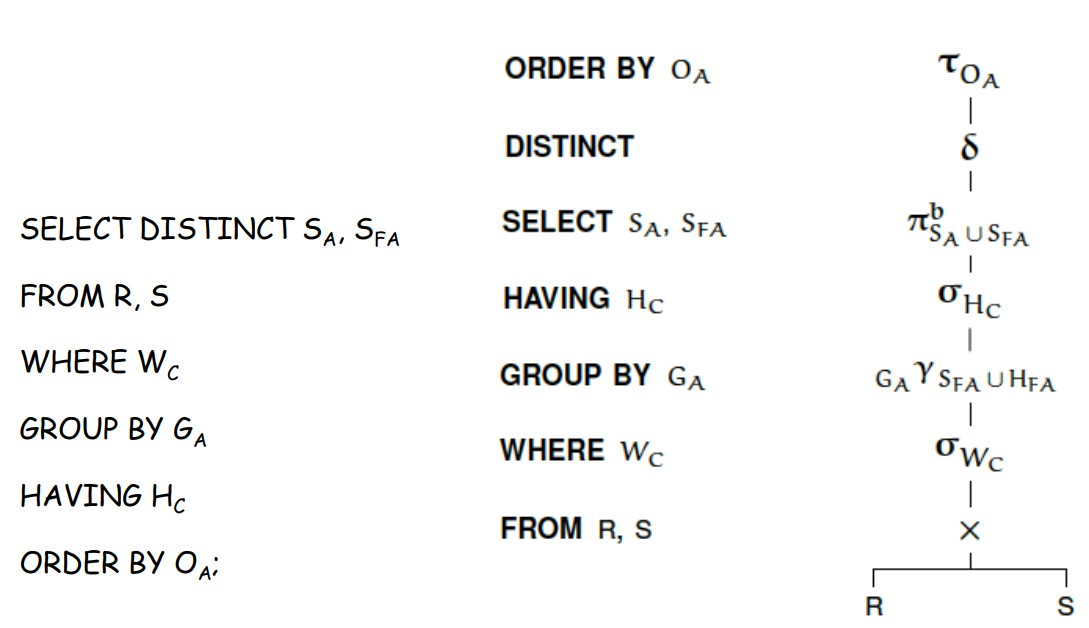
\includegraphics[width=\textwidth]{immagini/SQL_alRel.jpg}
	\caption*{Confronto fra SQL e Algebra relazionale}
\end{figure}

\subsubsection{Riferimento alle colonne}
Spesso nel riferimento alle colonne selezionate nel join è necessario specificare da quale delle tabelle la colonna è stata estratta, al fine di evitare ambiguità.\
La sintassi usata è ``\texttt{NomeTabella.NomeColonna}''.

\subsubsection{Ridenominazioni}

Di solito in una \texttt{select} che definisce una join possono essere necessarie ride\-nominazioni
\begin{itemize}
	\item nel prodotto cartesiano (ossia ridenominare le tabelle coinvolte),
	\item nella target list (ossia ridenominare gli attributi).
\end{itemize}

\subsection{Join}

Se due tabelle del database contengono dei dati in comune, possono essere correlate mediante un'operazione di \textit{join}.\
Le colonne delle due tabelle che creano la correlazione rappresentano la stessa entità, ossia i loro valori appartengono allo \textbf{stesso dominio}.\
In genere le colonne delle due tabelle considerate sono legate da un vincolo di chiave esterna (ma non è obbligatorio).

Il \textbf{join} (o \textbf{equi-join}) fra due tabelle è una terza tabella le cui righe sono tutte e sole quelle ottenute dal prodotto cartesiano delle righe delle due tabelle di partenza i cui valori delle colonne espresse dalla condizione di join sono uguali.\
In SQL il join viene realizzato mediante una particolare forma del \texttt{SELECT}, in cui nella clausola \texttt{FROM} vengono indicate le due tabelle coinvolte e nella clausola \texttt{WHERE} viene espresso il collegamento fra le due tabelle, mediante la condizione di join.

\begin{flushleft}
	$\mathtt{Tab_1(A_1,A_2)\ Tab_2(A_3,A_4)}$

	\quad $\mathtt{SELECT\ Tab_1.A_1, Tab_2.A_4}$

	\quad $\mathtt{FROM\ Tab_1, Tab_2}$

	\quad $\mathtt{WHERE\ Tab_1.A_2 = Tab_2.A_3}$
\end{flushleft}

\noindent Traduce l'espressione dell'algebra relazionale
\[\pi_{\mathrm{A_1,A_4}} (\sigma_{\mathrm{A_2=A_3}} (\mathrm{Tab_1} \Join \mathrm{Tab_2}))\]

\noindent Quindi il join consiste di un prodotto cartesiano (\texttt{FROM}), di una selezione (\texttt{WHERE}) e di una proiezione (\texttt{SELECT}).

La condizione di join può essere presente assieme ad altre condizioni mediante il connettore logico \texttt{AND}.

Se si vogliono selezionare tutte le colonne delle due tabelle si può sempre usare la notazione ``\verb|nome_tabella.*|''.

\paragraph{Inner-Join}
È un'operazione di join in cui la condizione non sia necessariamente una condizione di uguaglianza.\

\subsubsection{Self-Join}

Un caso molto particolare di Join è quello che mette in relazione una tabella con se stessa.\
Questo si può ottenere ridenominando due volte la tabella con due nomi diversi, trattando le due copie come se si trattasse di due tabelle diverse.\
In questo caso si parla di \textbf{Self Join}.

\begin{flushleft}
	$\mathtt{SELECT\ X.A_1, Y.A_4}$

	$\mathtt{FROM\ Tab_1\ X, Tab_2\ Y, Tab_1\ Z}$

	$\mathtt{WHERE\ X.A_2 = Y.A_3\ AND\ X.A_2 = Z.A_1}$
\end{flushleft}

\subsubsection{Cross Join}

Talvolta un'interrogazione può coinvolgere più di due tabelle $\rightarrow$ il \textbf{cross-join} implementa il prodotto cartesiano.\
Si realizza semplicemente mediante una select che utilizza le due (o più) tabelle coinvolte, senza specificare nessuna condizione di join.

\subsubsection{Join On}

Oltre alla forma vista, nei DBMS più moderni, per effettuare il join di due tabelle è possibile utilizzare una forma più esplicita (standard ANSI).\ La sintassi è la seguente:
\begin{flushleft}
	\texttt{SELECT Attributi}

	$\mathtt{FROM\ Tab_1\ JOIN\ Tab_2}$

	\texttt{ON CondizioneDiJoin}
\end{flushleft}

\subsubsection{Equi-Join e Natural Join}

Se dobbiamo operare una \textbf{equi-join}, ossia un join la cui condizione sia una condizione di uguaglianza, e che sia anche un \textbf{Natural Join}, ossia un join creato su \textit{tutte} le colonne che hanno il medesimo nome in entrambe le tabelle, possiamo utilizzare la seguente sintassi:

\begin{flushleft}
	\texttt{SELECT listaAttributi}

	$\mathtt{FROM\ Tab_1\ NATURAL\ JOIN\ Tab_2}$
\end{flushleft}

\subsubsection{Using}

Può succedere comunque che nelle tabelle coinvolte ci siano più attributi con lo stesso nome, e col \texttt{Natural Join} tutte queste coppie di attributi presi dalla due tabelle vengono identificate.\
Se invece vogliamo operare una join in cui la condizione riguarda solo una o alcune di queste coppie, si usa la clausola \texttt{USING} seguita dall'elenco degli attributi coinvolti nella condizione:
\begin{flushleft}
	\texttt{SELECT lista attributi}

	$\mathtt{FROM\ Tab_1\ JOIN\ Tab_2}$2

	$\mathtt{USING\ (attr_1,attr_2,\dots)}$
\end{flushleft}

\subsubsection{Outer Join}
Quando vengono correlate mediante una join delle tabelle con colonne contenenti dati in comune, è possibile che un valore sia presente in una delle colonne e non nell'altra.\
Effettuando un equi-join la riga corrispondente a tale valore viene scartato.\

In alcuni casi invece può essere necessario mantenere questi valori.\
Per fare questo si deve effettuare un \textbf{outer join}.
\begin{flushleft}
	\texttt{SELECT lista\_attributi}

	$\mathtt{FROM\ Tab_1\ LEFT\ [OUTER]\ JOIN\ Tab_2}$
\end{flushleft}
\begin{flushleft}
	\texttt{SELECT lista\_attributi}

	$\mathtt{FROM\ Tab_1\ RIGHT\ [OUTER]\ JOIN\ Tab_2}$
\end{flushleft}
\begin{flushleft}
	\texttt{SELECT lista\_attributi}

	$\mathtt{FROM\ Tab_1\ FULL\ [OUTER]\ JOIN\ Tab_2}$
\end{flushleft}

L'operatore di \texttt{OUTER JOIN} può essere applicato usando la seguente sintassi:
\begin{itemize}
	\item \{\texttt{LEFT} $|$ \texttt{RIGHT} $|$ \texttt{FULL}\} \texttt{[OUTER] JOIN} + \texttt{ON} $\langle$predicato$\rangle$
	\item \{\texttt{LEFT} $|$ \texttt{RIGHT} $|$ \texttt{FULL}\} \texttt{[OUTER] JOIN} + \texttt{USING} $\langle$colonne$\rangle$
\end{itemize}
dove `\texttt{OUTER}' è opzionale.

\section{Sub-Query}

Una \textbf{subquery} è un comando \texttt{Select}, racchiuso tra parentesi tonde, inserito all'interno di un comando SQL, per esempio un'altra \texttt{Select}.\
Le subquery possono essere utilizzate nei seguenti casi:
\begin{itemize}
	\item in espressioni di confronto,
	\item in espressioni di confronto quantificato,
	\item in espressioni \texttt{IN},
	\item in espressioni \texttt{EXISTS},
	\item nel calcolo di espressioni.
\end{itemize}

Tre tipologie: scalare, di colonna, di tabella.\

\noindent \textbf{Subquery Scalare}:\ è un comando \texttt{Select} che restituisce un solo valore.
\begin{flushleft}
	\texttt{SELECT Max(Cilindrata) FROM Veicoli}

	\texttt{SELECT Cod\_Categoria FROM Veicoli Where Targa=``123456''}
\end{flushleft}

\noindent \textbf{Subquery di Colonna}:\ è un comando \texttt{Select} che restituisce una colonna
\begin{flushleft}
	\texttt{SELECT cod\_categoria FROM Veicoli}
\end{flushleft}

\noindent \textbf{Subquery di Tabella}:\ è un comando \texttt{Select} che restituisce una tabella
\begin{flushleft}
	\texttt{SELECT Targa, Cod\_mod, Posti FROM Veicoli}
\end{flushleft}

\noindent Inoltre si ricorda che nelle \texttt{Select} semplici non è possibile utilizzare contemporaneamente funzioni di gruppo e funzioni su singole righe, questo viene reso possibile mediante l'uso delle subquery.

\subsubsection{Quantificazione}

Tutte le interrogazioni su di una associazione multivalore vanno quantificate.
\begin{itemize}
	\item Universale negata = esistenziale
	\item Esistenziale negata = universale
\end{itemize}

\subsubsection{Any, All ed Exists}

Le condizioni in SQL permettono anche il confronto fra un attributo e il risultato di una subquery che restituisce una colonna o una tabella.

\noindent Operatore \textbf{Scalare} (\texttt{ANY} $|$ \texttt{ALL}) SelectQuery
\begin{itemize}
	\item \texttt{ANY}:\ il predicato è vero \textit{se almeno uno dei valori restituiti} dalla query soddisfano la condizione.
	\item \texttt{ALL}:\ il predicato è vero se tutti i valori restituiti dalla query soddisfano la condizione.
\end{itemize}
In particolare le forme \texttt{= ANY} (equivalentemente \texttt{IN}) e $\neq$ \texttt{ALL} (equivalentemente \texttt{NOT IN}), forniscono un modo alternativo per realizzare intersezione e differenza dell'algebra relazionale.\

Quantificatore \textbf{esistenziale}:\ \texttt{EXISTS} SelectQuery.\
Il predicato è vero se la SelectQuery \textit{restituisce almeno una} ennupla.\
Mediante \texttt{EXIXST(SELECT*\dots)} è possibile verificare se il risultato di una subquery resituisce almeno una tupla.\
Facendo uso di \texttt{NOT EXISTS} il predicato è vero se la subquery non restituisce alcuna Tupla.

Occorre un meccanismo per rendere più flessibile la clausola \texttt{exists}, rendendo le condizioni della subquery dipendenti dalla tupla della query principale (query esterna), quindi si introduce un legame fra la query e la subquery (query correlate) e si definisce una variabile (un alias) nella query esterna che si utilizza nella subquery.

\subsubsection{Semantica delle espressioni ``correlate''}

La query più interna può usare variabili della query esterna.\
L'interrogazione interna \textit{viene eseguita una volta per ciascuna ennupla} dell'interrogazione esterna.

Le subquery oltre che essere usate all'interno della clausola \texttt{WHERE}, possono anche essere utilizzate nel calcolo di espressioni, dunque per definire colonne.\

\section{Unione, Intersezione, Differenza}

A volte può essere utile poter ottenere un'unica tabella contenente alcuni dei dati contenuti in due tabelle omogenee, ossia con attributi definiti sullo stesso dominio.\
Per esempio:\ operazioni booleane, calcolando unione, intersezione e differenza.

In SQL la \texttt{SELECT} da sola non permette di fare questo tipo di operazioni su tabelle.\
Esistono per questo dei costrutti espliciti che utilizzano le parole chiave

\begin{flushleft}
	\texttt{UNION}

	\texttt{INTERSECT}

	\texttt{EXCEPT} (in oracle \texttt{MINUS})
\end{flushleft}
Tali operatori lavorano sulle tabelle come se fossero insiemi di righe, dunque i duplicati vengono eliminati (a meno che si usi la specifica \texttt{ALL}) anche dalle proiezioni!

\subsubsection{Unione}

L'operatore \texttt{UNION} realizza l'operazione di unione definita nell'algebra relazionale.\
Utilizza come operandi le due tabelle risultanti da comandi \texttt{SELECT} e restituisce una terza tabella che contiene \textbf{tutte le righe della prima e della seconda tabella}.\
Nel caso in cui dall'unione e dalla proiezione risultassero delle righe duplicate, l'operatore \texttt{UNION} ne mantiene una sola copia, a meno che non sia specificata l'opzione \texttt{ALL} che indica la volontà di mantenere i duplicati
\begin{flushleft}
	\texttt{SELECT\ \dots}

	\texttt{UNION [ALL]}

	\texttt{SELECT\ \dots}
\end{flushleft}

\noindent Quali nomi per gli attributi del risultato?
\begin{itemize}
	\item nessuno
	\item quelli del primo operando
	\item \dots
\end{itemize}
In SQL quelli del primo operando.

Quanto detto riguardo alla \textit{notazione posizionale} dell'operatore \texttt{UNION} vale equivalentemente per gli altri operatori booleani \texttt{EXCEPT} (\texttt{Minus} in Oracle) e \texttt{INTERSECT}.

\subsubsection{Differenza}

L'operatore \texttt{EXCEPT} utilizza come operandi due tabelle ottenute mediante due \texttt{select} e ha come risultato una nuova tabella che contiene \textbf{tutte le righe della prima che non si trovano nella seconda}:\ realizza la differenza dell'algebra relazionale.\
Anche qui si può specificare l'opzione \texttt{ALL} per indicare la volontà di mantenere i duplicati.\
Sintassi:

\begin{flushleft}
	\texttt{SELECT\ \dots}

	\texttt{EXCEPT [ALL]}

	\texttt{SELECT\ \dots}
\end{flushleft}

\noindent Nota che la differenza può essere effettuata da un'unica select che utilizza subselect.\

\subsubsection{Intersezione}

L'operatore \texttt{INTERSECT} utilizza come operandi due tabelle risultanti dai comandi \texttt{SELECT} e restituisce una tabella che contiene le righe comuni alle due tabelle iniziali.\
Realizza l'intersezione dell'algebra relazionale.\
Sintassi:
\begin{flushleft}
	\texttt{SELECT\ \dots}

	\texttt{INTERSECT [ALL]}

	\texttt{SELECT\ \dots}
\end{flushleft}
L'opzione \texttt{ALL} serve a mantenere gli eventuali duplicati di righe.\
In sua assenza, si mantiene una sola copia delle righe duplicate.

\section{SQL per la modifica di basi di dati}

Introduciamo ora il \textbf{Data Manipulation Language} (\textbf{DML}) ossia il linguaggio SQL che serve per \textbf{inserire}, \textbf{modificare} e \textbf{cancellare} i dati del database, ma anche per \textbf{interrogare il database}, ossia estrarre i dati dal database.\

Inizialmente descriveremo le istruzioni che servono a inserire, cancellare e modificare i dati.\
In seguito introdurremo le istruzioni per estrarre dal database le informazioni che ci interessano.

\subsubsection{Insert}
Supponiamo di volere inserire un nuovo dato in una tabella.\
Tale operazione si realizza mediante l'istruzione
\begin{center}
	\texttt{INSERT INTO \dots VALUES}
\end{center}
Sintassi:
\begin{flushleft}
	\texttt{INSERT INTO nome tabella}

	$\mathtt{[(ListaAttributi)]\ VALUES\ (ListaDiValori)}\ |$

	\texttt{SQLSelect}
\end{flushleft}

\noindent Ai valori non attribuiti viene assegnato \texttt{NULL}, a meno che non sia specificato un diverso valore di default.\
L'inserimento fallisce se \texttt{NULL} non è permesso per gli attributi mancanti.\
Non specificare gli attributi equivale a specificare tutte le colonne della tabella.\
\textbf{Nota bene}:\ si deve rispettare l'ordine degli attributi.

È possibile effettuare un insert prendendo i dati da un'altra tabella mediante il comando di interrogazione del database \texttt{SELECT}:\ con questo tipo di insert si possono effettuare tanti inserimenti simultaneamente.\

\subsubsection{Delete}

Per eliminare un elemento bisogna individuare quale.\
Questo si può stabilire mediante la clausola \texttt{WHERE}, dove viene stabilita una condizione che individua l'elemento (o gli elementi) da cancellare.\
Spesso un particolare elemento può essere individuato mediante il suo valore nella chiave primaria.

\noindent Sintassi
\begin{flushleft}
	\texttt{DELETE FROM nome\_tabella}

	\texttt{[WHERE Condizione]}
\end{flushleft}

\noindent La condizione del delete può essere una normale condizione di \texttt{SELECT}.\
Questa modalità di delete permette di cancellare più righe con un'unica istruzione, purché le righe soddisfino la condizione.\

\subsubsection{Update}

Inoltre è possibile aggiornare alcuni dati seguendo la seguente sintassi:

\begin{flushleft}
	\texttt{UPDATE Tabella}

	\texttt{SET Attributo = Espr}

	\texttt{WHERE Condizione}
\end{flushleft}
